\documentclass{article}
\usepackage[utf8]{inputenc}
\usepackage[T1]{fontenc}
\usepackage[english]{babel}
\usepackage{amsthm}
\usepackage{parskip}
\usepackage{algorithmicx}
\usepackage{amsmath}
\usepackage{algorithm}
\usepackage{algpseudocode}

\usepackage{graphicx}
\graphicspath{ {images/} }
\title{Spanning trees in strongly connected graphs with per-vertex degree constraints}
\date{2018 June}
\author{Samuel Chase}
\begin{document}
	\maketitle
	\section{Introduction}
	In this project, I sought to develop and prove new algorithms to create spanning trees in general graphs with per-vertex constraints. 
	This means that each vertex in the graph would have some additional value, a degree constraint $d$. For a spanning tree to be correct every vertex in the spanning tree must have a degree exactly equal to that degree constraint $d$. This poses an additional constraint on what
	would otherwise be a trivial spanning tree problem. In this paper two proofs will be discussed and analyzed, which inspired my studies and led to the development of the algorithm for determining a spanning tree on strongly connected graphs. It is my hope that in the future this algorithm can be modified to apply to the general case.
	
	
	
	\section{Fast vertex cover with double star graphs \\ {\large Based on \textit{Covering by trees of small diameter} by Lov\'asz}}
	In his paper \textit{Covering by trees of small diameter}, Lov\'asz discusses double star trees. A graph's diameter is the maximum number of edges to connect any two vertices in the graph. Double star trees are trees of diameter less than or equal to 3. A double star can be formed by taking any two star graphs, graphs featuring a central node with any number of edges connected only to that central node, and adding an edge between the central nodes of the two stars, as seen in Figure 1
	\begin{figure}[h]
		\caption{}
		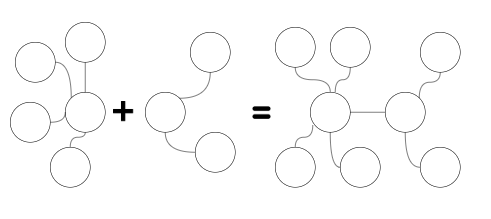
\includegraphics{Figure1}
	\end{figure}
	
	Double stars also have the interesting property of being able to cover grap hs incredibly quickly. In fact, a graph of $n$ vertices be covered by a greedy algorithm taking at most $2n/3$ steps. All that is required to cover a graph with double stars is to find a maximal matching of edges (A set of edges $E$ such that no edge can be added without touching a vertex already touched by $E$), and then add double stars centered around those edges, where the two vertices connected to the edge form the individual single stars. Lov\'asz has proved this to be true, and that $2n/3$ double stars are required. Discussed in this paper will be the key determinants in a maximal double-star cover, as well as examples of such covers on simple graphs.
	\subsection{The algorithm}
	
	Lov\'asz begins by asserting that $\tau$ is the maximum number of TODO DEFINE independent vertices of $G$. He also states that $M$ as the maximal matching of $G$, having size $r$. $I$ is defined as the vertices not covered by $M$, with a size of $s$. If $n$ = $2r$ then $I$ = $\emptyset$.
	\\\\
	In section 2 it is stated that $f_{3}(g)$ is the maximum number of double stars required to cover a graph. We also know $f_{3}(g) \leq f_{2}(g)$ as in the worst case it is still impossible that double stars cover worse than single stars. This leads Lov\'as to know that $n-\tau \leq n-s = 2r$, or the number of vertices minus independent vertices is less than or rqual to the vertices minus the vertices consained in $I$, which is equal to the number of vertices in $M$.
	\\\\
	In section 3 Lov\'asz moves on to looking at $S_{i}$. $S_{i}$ is a double star of parts of $M$. $T_{i}$ is the tree of all edges containing $c_{i}$ (from $i$). We know that the set of all $S$ and $T$ covers $G$, therefore $f_{3}(g) \leq r + s = n - r$, or the maximum number of double stars required to cover a graphis less than or equal to the size of $m$ plus the size of $i$, which is equal to the size of $g$ minus the size of $m$.
	\\\\
	Combining what is learned in section 4 we are able to prove Lov\'asz's theorem, that $f_{3}(g) \leq 2n/3$
	
		\subsection{Examples}
		Presented below are examples of graphs of various sizes. It may be noted that some of these graphs themselves are double stars. This reveals some of the inefficiency with this algorithm - even when a small cover (potentially even one of size 1) is available a larger cover may be selected simply because of the nature of the greedy algorithm. Similarly, the steps taken will be laid out sequentially, and if different edges are selected the end cover might be very different.
		 \\
				\begin{figure}[H]
				\caption{}
				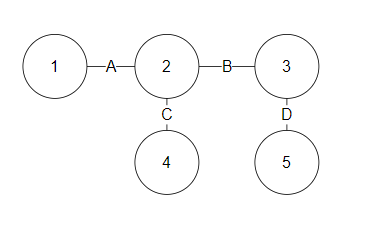
\includegraphics{Figure2}
			\end{figure}
		\\
			Above, in figure 2, we see a double star graph. We know that $n$ is equal to 5. Running our greedy algorithm to find a maximal matching, we will assume we select edges c and d. This means $M = \{c,d\}$, and therefore $r = 2$. $I$ will be all vertices not touched by $M$, therefore $I = \{1\}$ and $s$ = 1. Knowing that $f_{3}(g) \leq n-r$, we can say that the maximum number of double stars necessary to cover this graph is 3. An example of this maximum cover is a cover containing double stars centered around a,b, and c. Assuming we make the odd choice of selecting $a$ and $c$ to be the centers of our first two double stars, we notice that if we add either $b$ or $d$ we will necessarily have a full cover. Although this is something our algorithm would never provide as a cover (due to $a$ and $b$ being adjacent) this shows a theoretical maximum size for the vertex cover. It is simply impossible to increase this value, knowing that no matter which edges we choose in any order we will cover the graph in at most 3 double stars.
	\newtheorem{theorem}{Theorem}
	\section{Spanning trees in connected graphs with per-vertex degree constraints}
	Assume that we wish to create a spanning tree for a graph. Correct algorithms for this problem proven by Kruskal and other
	mathematicians, however in this case we wish to consider an additional constraint. Assume that in the graph every vertex has some degree constraint $d$,
	where for a spanning tree to be correct every vertex in the spanning tree must have a degree exactly equal to that degree constraint $d$. 
	\\\\
	An algorithm for solving this problem can be seen below:
	\\
		\begin{algorithm}[H]
		\caption{Creating a spanning tree on a graph with per-vertex degree constraints}
		\begin{algorithmic}[1]
			\State Graph $G(V,E)$ with a total degree of 2n-2 where n is the magnitude of $V$
			\State T = $\emptyset$
			\State T += ($v1$,$v2$) where $v1$ is the vertex of largest degree in V, and $v2$ is the vertex of second largest degree. Decrement the degree of $v1$ and $v2$
			\While{There exits a vertex in $V$ and $T$ with a degree $>$ 0 }
			\State {T+= ($t$,$v$) where $t$ is the vertex of largest degree in $t$, and $v$ is the largest vertex in $V$\textbackslash$T$}
			\EndWhile
		\end{algorithmic}
	\newpage
	\end{algorithm}

	\begin{theorem}
		Given a strongly connected graph $G(E,V)$ with total vertex degree constraint of $2(|V|-1)$ algorithm 2 will return a correct spanning tree
	\end{theorem}

	\begin{proof}
		Allow the algorithm to run until step 3, producing tree $T$. $G \setminus T$ will have a total degree constraint of $2(|V|-1)-2$, accounting for the single edge in T. Therefore, because it has a total degree constraint of $2(|V|-2)$ and needs to connect $|V|-2$ vertices to $T$. Thus the spanning tree will be able to be completed as the number of possible edges is equal to twice the number of vertices, and $T$ will either have a total degree constraint $\geq$ 1, or be $G$. 
		\\
		\\
		Now, assume $T$ has grown to size k vertices correctly, where $T$ has a total degree constraint large enough to complete the spanning of the graph
		\\\\
		$T$ will now select the next untouched vertex of maximum degree. There are 3 cases for this vertex:
		
		\setlength\parindent{12pt} 
		Case 1) The next vertex selected has a degree = 1 \par
		\setlength\parindent{24pt}\hangindent=24pt 
		In this case, if the largest vertex remaining has a degree constraint of 1 then all vertices not in $T$, $U$, must
		have a degree constraint of 1. Thus $T$ must have a total remaining vertex constraint of $|V \setminus U|$, which is equal to  $|U|$. Therefore as there are $|U|$ vertices not in $T$ and $T$ has a total degree constraint of $|U|$ we know the degree constraint will not be violated, as each connection from $T$ to $U$ lowers the total degree constraint by one.  Thus $T$ will be able to complete the spanning tree.
		\par
		
		\setlength\parindent{12pt}
		Case 2) The next vertex selected has a degree $\geq$ 1\par
		\setlength\parindent{24pt}\hangindent=24pt 
		Adding this vertex to $T$ will increase $T$'s total degree constraint by some value $\geq$ 2, and then decrease $T$'s total degree constraint by 2.
		Therefore the change in $T$ cannot be less than zero, and thus $T$ will not be decreased and therefore $T$ will be able to complete the spanning tree.
		\par
		
		
		\setlength\parindent{12pt}
		Case 3) No new vertex can be selected\par
		\setlength\parindent{24pt}\hangindent=24pt 
		If no new vertex can be selected this means every vertex in $G$ is in $T$. Thus the spanning tree will be completed.
		\par
		
		\setlength\parindent{0pt}\hangindent=0pt
		Therefore it is clear that $T$ will not violate degree constraints at every step of the algorithm,
		
	\end{proof}		

\end{document}
